\section{Auswertung}
Zunächst wird das Signal des Funktionsgenerators überprüft. Am Ausgang des Refernece/Oscillator liefert
die sinusförmige Referenzspannung eine konstante Amplitude von $3,28 \, \si{\volt}$.

Zur Überprüfung welches Signal am Mischer ankommt wird ein sinusförmiges Signal $U_\text{sig}$ mit
einer Frequens $\omega = 1 kHz$ und einer Amplitude von $10 \, mV$ eingestellt.

Eine schematische Darstellung der Amplitude in unterschiedlichen Phasen zeigt die nun folgenden
Bildschirmfotos dar.
\begin{figure}[H]
\centering
\begin{subfigure}{0.48\textwidth}
	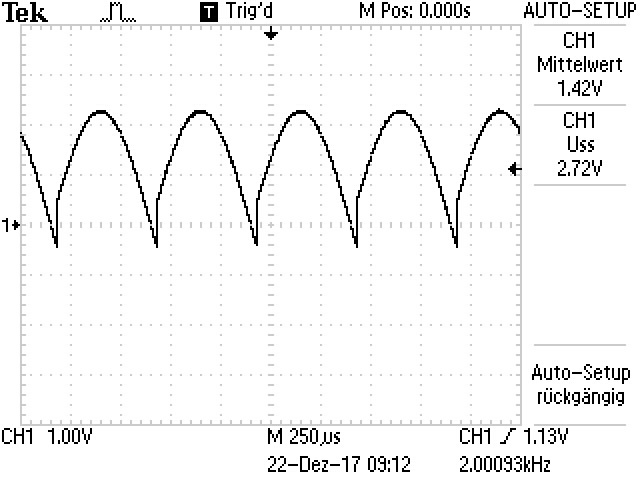
\includegraphics[width=\textwidth]{0Grad.JPG}
  \subcaption{Phasendifferenz bei 0 Grad}
\end{subfigure}
\begin{subfigure}{0.48\textwidth}
  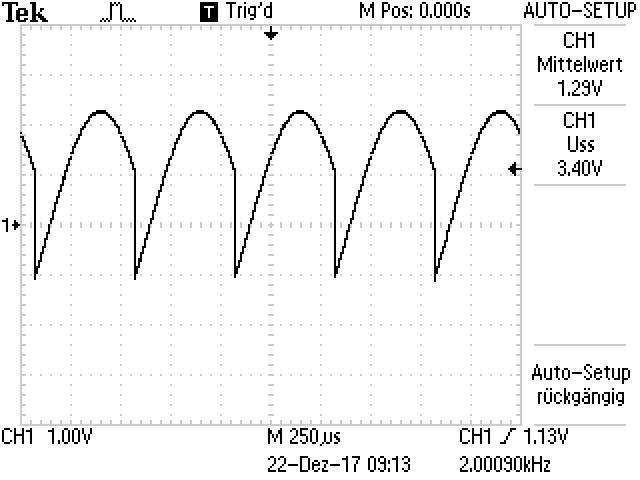
\includegraphics[width=\textwidth]{45Grad.JPG}
  \subcaption{Phasendiffernez bei 45 Grad}
\end{subfigure}
\begin{subfigure}{0.48\textwidth}
	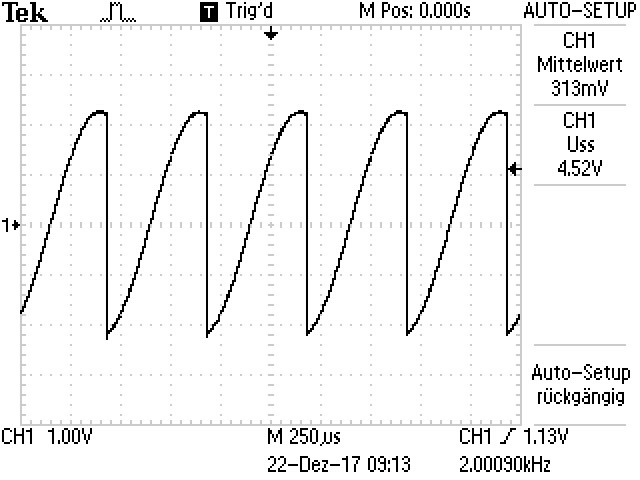
\includegraphics[width=\textwidth]{90Grad.JPG}
  \subcaption{Phasendifferenz bei 90 Grad}
\end{subfigure}
\begin{subfigure}{0.48\textwidth}
  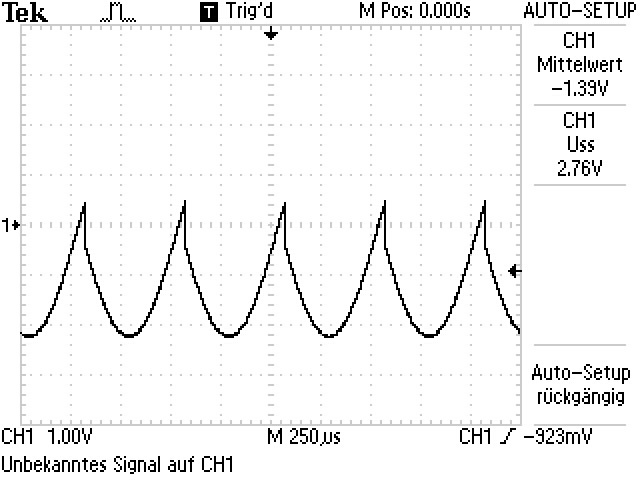
\includegraphics[width=\textwidth]{180Grad.JPG}
  \subcaption{Phasendiffernez bei 180 Grad}
\end{subfigure}
\begin{subfigure}{0.48\textwidth}
	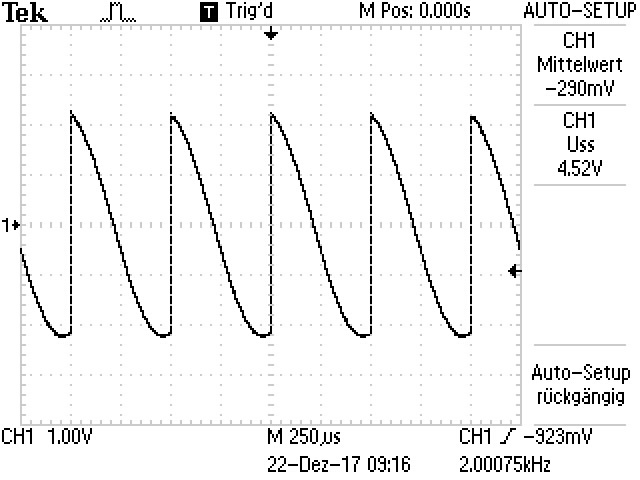
\includegraphics[width=\textwidth]{270Grad.JPG}
  \caption{Phasendifferenz bei 270 Grad}
\end{subfigure}
\end{figure}

Anschließend wird das Signal am Mischer durch ein Tiefpassfilter angeschlossen und folgende
Messwerte sind in der Tabelle (\ref{tab:1}) dargestellt.
Die Theoriewerte werden mit der Gleichung (\ref{eq:1}) berechnet.
$U_o$ ist durch den Vorverstärker und Verstärker auf $55,6 V$ verstärkt worden.\\
Im Diagramm (\ref{abb:5}) wurde ein Ausgleichsrechnung durchgeführt, da die eingestellte Phasenverschiebung
nicht geeicht war. Die Ausgleichsrechnung wurde mithilfe von Python 3.6 durchgeführt.
\begin{figure}[H]
	\centering
	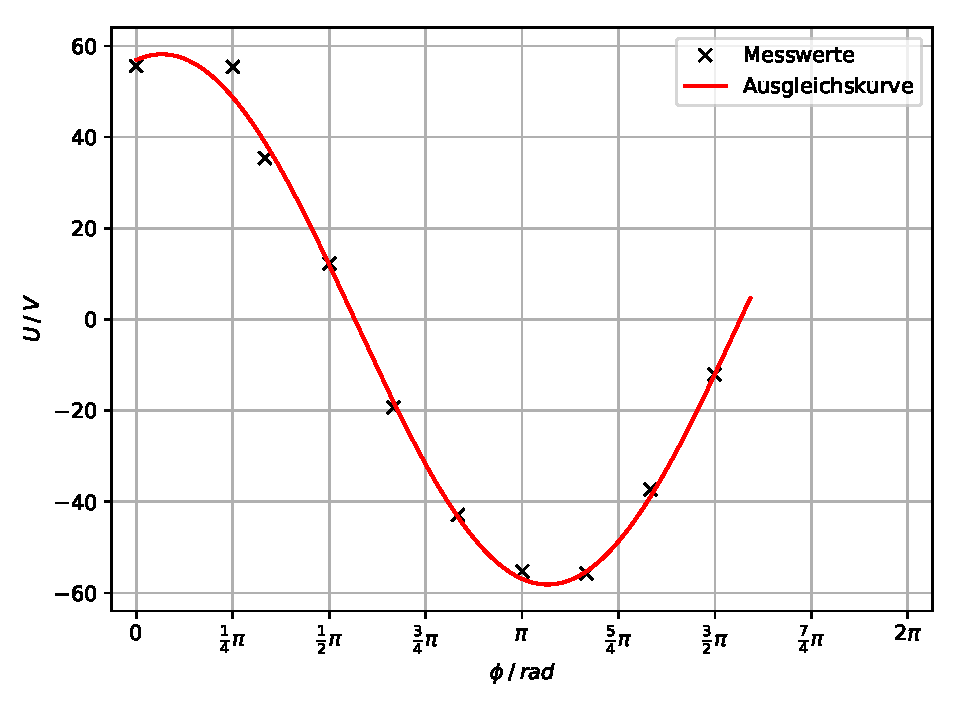
\includegraphics[width=\textwidth]{kurve1.pdf}
	\caption{Darstellung der Referenzspannung.}
	\label{abb:5}
\end{figure}
Folgende Ausgleichsrechnung wurde angewandt:
\begin{equation}
	 U_o = A \cdot cos(x - \phi)
	 \label{eq:10}
 \end{equation}
Dabei ist $A$ die Amplitude, $x$ die eingestellte Phase und $\phi$ die Phasenverschiebung.
\begin{itemize}
	\item $A = \SI{58.3(14)}{\volt}$
	\item $\phi = (\num{0.205(30)}) \, \text{rad}$
\end{itemize}
\begin{table}[H]
\centering
\caption{Darstellung der Messergebnisse.}
\label{tab:1}
 \begin{tabular}{c c c c}
  \toprule
     $U_\text{mess} / V$ & $\Phi/\circ$ & $U_\text{theo}$ & $Abweichung / \%$ \\
  \midrule
  55,6  & 0    & 54,36 & 2,28\\
  55,4  & 45   & 46,51 & 19,1\\
  35,4  & 60   & 37,03 & 4,40\\
  12,3  & 90   & 11,30 & 8,85\\
  -19,4 & 120  &-17,40 & 11,5\\
  -42,9 & 150  &-41,48 & 3,42\\
  -55,3 & 180  &-54,44 & 1,58\\
  -55,8 & 210  &-52,80 & 5,68\\
  -37,3 & 240  &-37,01 & 0,78\\
  -12,1 & 270  &-11,34 & 8,47\\
  \bottomrule
\end{tabular}
\end{table}

Nun wird ein Rauschsignal hinzugeschaltet. Das Verfahren erneut durchgeführt.
Eine schematische Darstellung der Amplitude mit Rauschen in unterschiedlichen Phasen wird in den nun folgenden
Bildschirmfotos gezeigt.

\begin{figure}[H]
  \centering
  \begin{subfigure}{0.48\textwidth}
	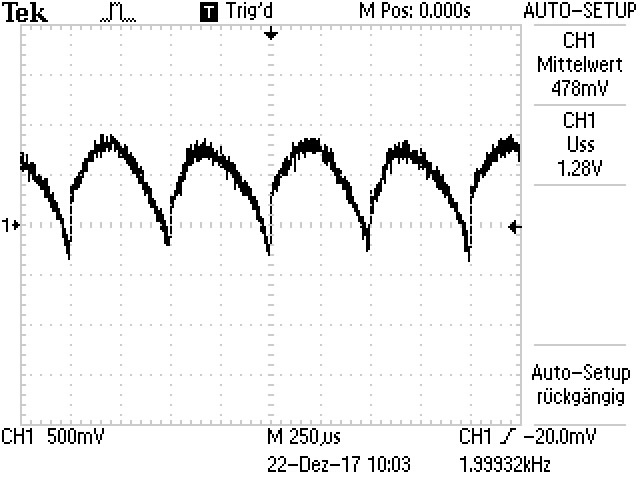
\includegraphics[width=\textwidth]{0GradR.JPG}
  \subcaption{Phasendifferenz bei 0 Grad}
\end{subfigure}
\begin{subfigure}{0.48\textwidth}
  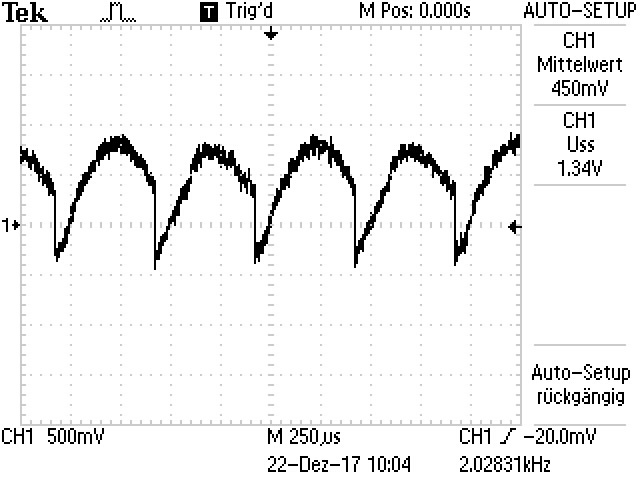
\includegraphics[width=\textwidth]{45GradR.JPG}
  \subcaption{Phasendiffernez bei 45 Grad}
\end{subfigure}
\begin{subfigure}{0.48\textwidth}
	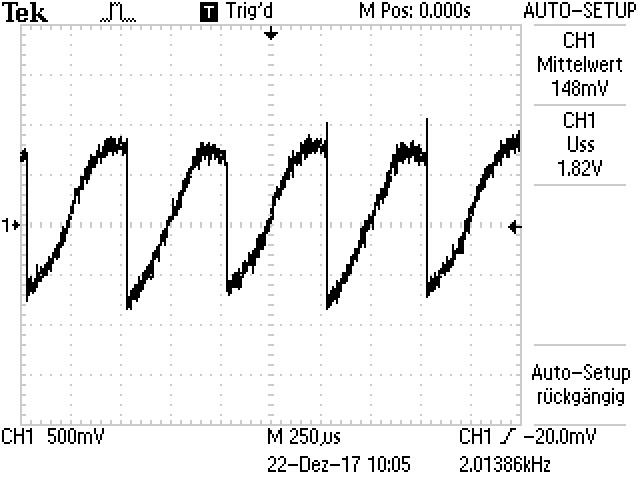
\includegraphics[width=\textwidth]{90GradR.JPG}
  \subcaption{Phasendifferenz bei 90 Grad}
\end{subfigure}
\begin{subfigure}{0.48\textwidth}
  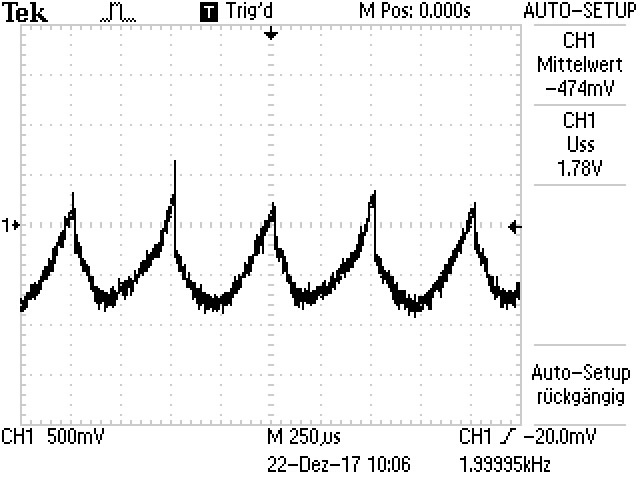
\includegraphics[width=\textwidth]{180GradR.JPG}
  \subcaption{Phasendiffernez bei 180 Grad}
\end{subfigure}
\begin{subfigure}{0.48\textwidth}
	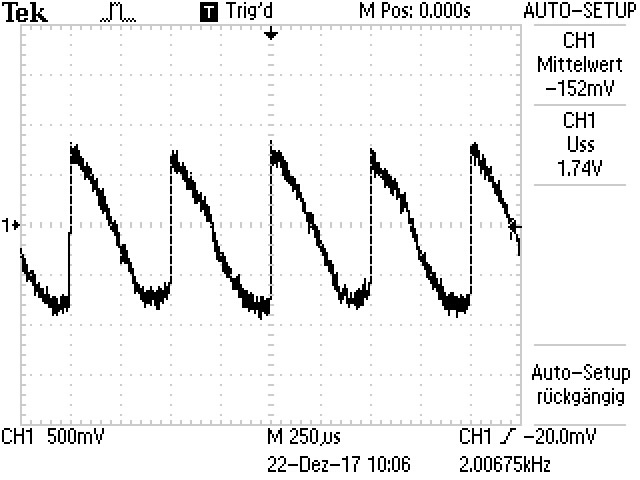
\includegraphics[width=\textwidth]{270GradR.JPG}
  \caption{Phasendifferenz bei 270 Grad}
\end{subfigure}
\end{figure}

Anschließend wird das Signal mit Rauschen an einen Tiefpassfilter angeschlossen und die
Messwerte sind in der Tabelle (\ref{tab:2}) dargestellt.
Auch bei diesem Fall wird mit Python 3.6 eine Ausgleichsrechnung durchgeführt,
welche in Abbildung (\ref{abb:8}) Graphisch dargestellt ist.\\\\

Diese Ausgleichsrechnung wurde wieder mit der Gleichung (\ref{eq:10}) durchgeführt.
In diesem Fall ergeben sich für die Parameter:

\begin{itemize}
	\item $A = \SI{50.55(152)}{\volt}$
	\item $\phi = (\num{0.311(3)}) \, \text{rad}$
\end{itemize}

\begin{table}[H]
\centering
\caption{Darstellung der Messergebnisse für das verrauschte Signal.}
\label{tab:2}
 \begin{tabular}{c c c c}
  \toprule
     $U_\text{mess} / V$ & $\Phi/\circ$ & $U_\text{theo} / V$ & $Abweichung/ \%$ \\
  \midrule
  49,2  & 0  & 	48,13 & 2,22 \\
  49,6  & 45 &  44,98 & 10,27 \\
  33,8  & 60 &  37,47 & 9,79 \\
  14,6  & 90 &  15,46 & 5,56 \\
  -4,12 & 120& -10,65 & 61,31 \\
  -36,7 & 150& -33,94 & 8,13 \\
  -47,8 & 180& -48,13 & 0,69 \\
  -49,6 & 210& -49,41 & 0,38 \\
  -34,5 & 240& -37,45 & 7,88 \\
  -14,6 & 270& -15,48 & 5,68 \\
  \bottomrule
\end{tabular}
\end{table}

\begin{figure}[H]
	\centering
	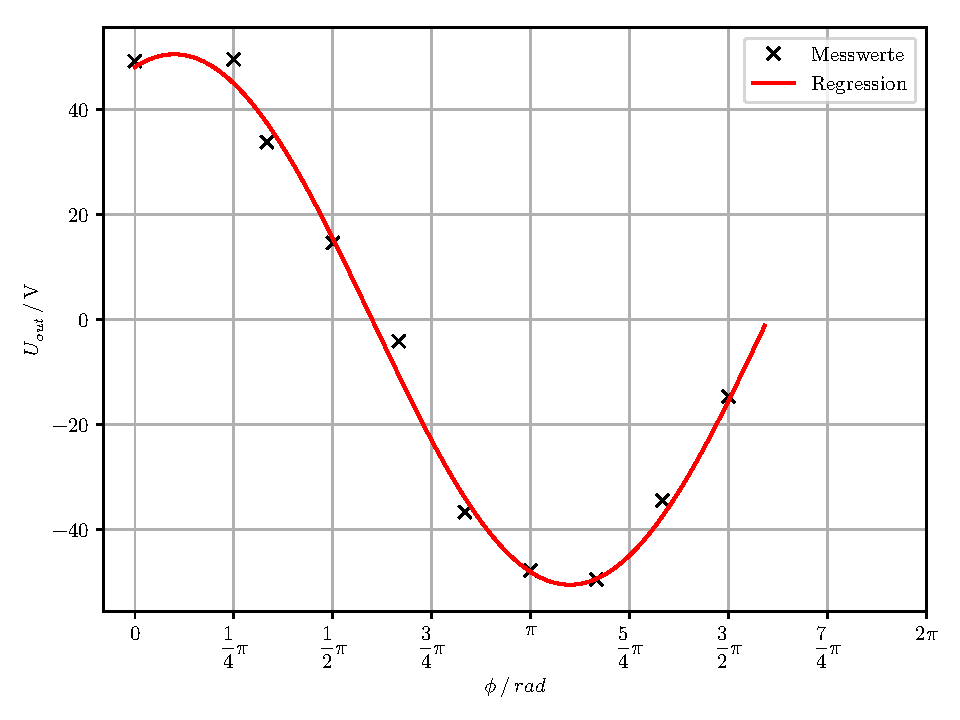
\includegraphics{plot5.pdf}
	\caption{Graphische Darstellung der Messwerte mit dem Rauschsignal.}
	\label{abb:8}
\end{figure}


Die Abweichung in Tabelle (\ref{tab:1}) und (\ref{tab:2}) sind mit folgende Formel
\begin{equation*}
  \sigma = \biggl| \frac{U_{theo}-U_\text{mess}}{U_{theo}} \biggl| \cdot 100
\end{equation*}
berechnet worden.

Bei der Leuchtdiode wird eine Rechteckspannung moduliert. Die eingestellte Frequenz ist $\omega = 159,6 \, \si{\hertz}$ und
besitzt eine Amplitude von $\SI{2}{\volt}$.
Folgende Messwerte werden in der Tabelle (\ref{tab:3}) und in der Abbildung (\ref{abb:6}) als
Diagramm dargestellt.

\begin{table}[H]
\centering
\caption{Messreihe zur Leuchtdiode}
\label{tab:3}
 \begin{tabular}{c c| c c}
  \toprule
     $Intensität / V$ & $r / cm$ &  $Intensität / V$ & $r / cm$  \\
  \midrule
  4,19 & 2,5 & 2,08 & 30,5  \\
  4,44 & 3,5 & 1,84 & 32,5  \\
  4,71 & 4,5 & 1,44 & 37,5  \\
  4,98 & 5,5 & 1,14 & 42,5  \\
  5,28 & 6,5 & 1,03 & 47,5  \\
  5,55 & 7,5 & 0,82 & 52,5  \\
  5,68 & 8,5 & 0,73 & 57,5  \\
  5,92 & 9,5 & 0,66 & 62,5  \\
  6,20 & 10,5& 0,60 & 67,5  \\
  6,37 & 11,5& 0,56 & 72,5  \\
  6,55 & 12,5& 0,65 & 77,5  \\
  6,65 & 14,5& 0,54 & 82,5  \\
  6,15 & 16,5& 0,49 & 87,5  \\
  5,02 & 18,5& 0,44 & 92,5  \\
  4,24 & 20,5& 0,32 & 102,5 \\
  3,58 & 22,5& 0,27 & 112,5 \\
  3,06 & 24,5& 0,20 & 122,5 \\
  2,48 & 26,5& 0,16 & 132,5 \\
  2,32 & 28,5&   -  &  -    \\
  \bottomrule
\end{tabular}
\end{table}

\begin{figure}[H]
  \centering
	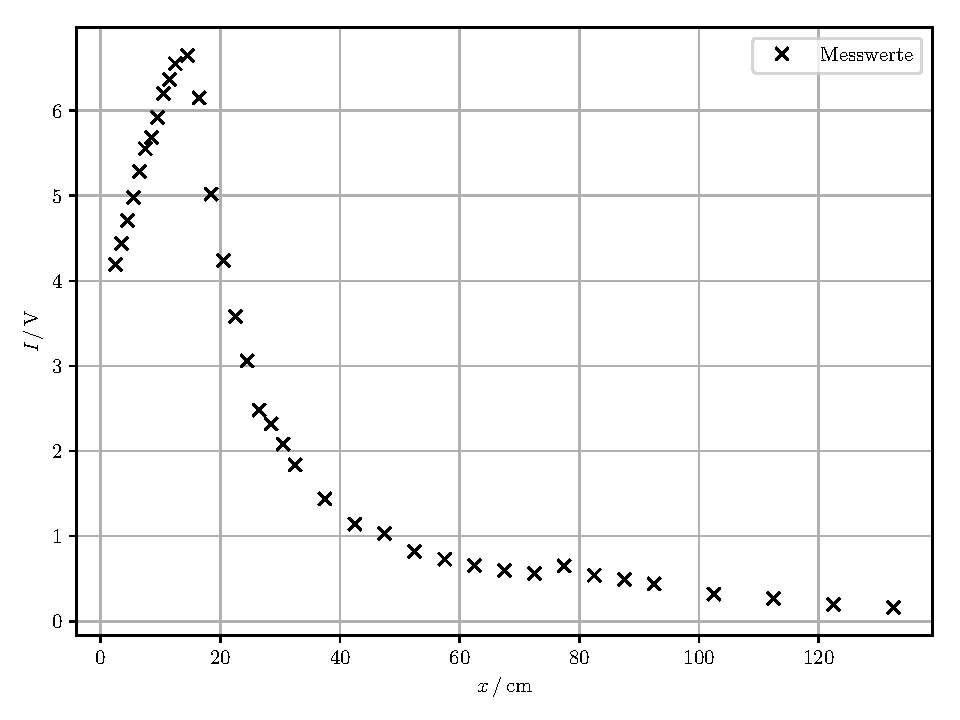
\includegraphics[width=\textwidth]{plot1.pdf}
  \caption{Darstellung der Intensität in Abhängigkeit des Abstandes}
  \label{abb:6}
\end{figure}

Die Werte bis zu dem Abstand $r = 14,5 \, cm$ sind physikalische nicht sinnvoll, nach
dem Gesetz der Strahlungsintensität. Dieses besagt, dass $I \propto \frac{1}{r^2}$ ist.
Daher werden die Messergebnisse ab dem Abstand von $r = 14,5 \, cm$ betrachtet und erneut in
Diagarmm (\ref{abb:7}) dargestellt.

\begin{figure}[H]
\centering
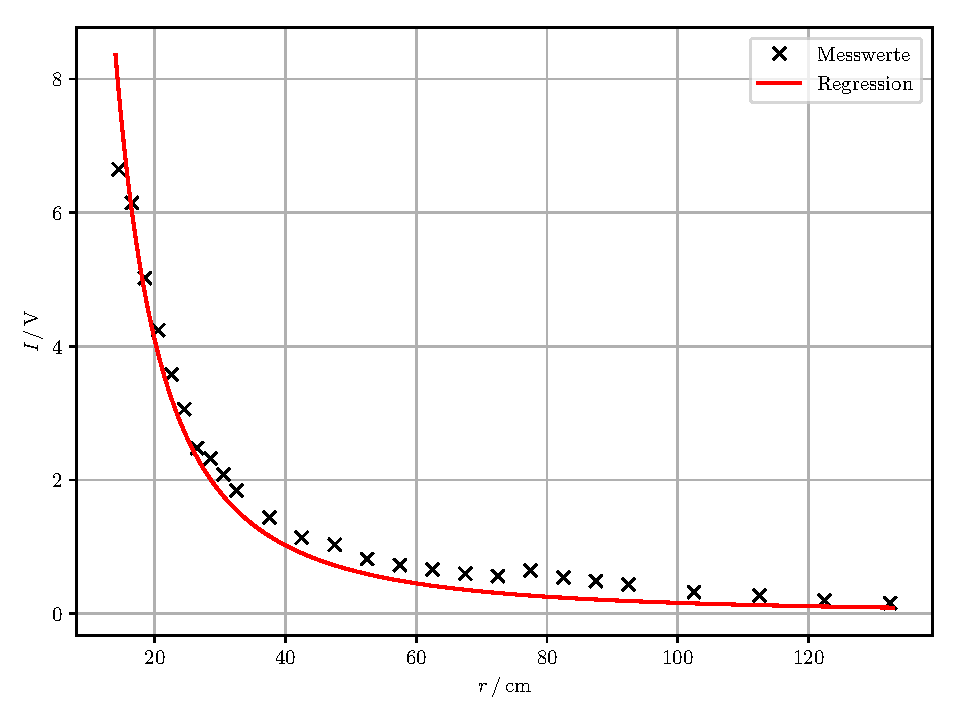
\includegraphics[width=\textwidth]{plot4.pdf}
\caption{Darstellung der Intensität in Abhängigkeit des Abstandes}
\label{abb:7}
\end{figure}
